\documentclass{article}
% translate with >> pdflatex -shell-escape <file>

% This file is used as unit test for pgfplots, copyright by Christian Feuersaenger.
% 
% See
%   http://pgfplots.sourceforge.net/pgfplots.pdf
% for pgfplots.
%
% Any required input files (for <plot table> or <plot file> or the table package) can be downloaded
% at
% http://www.ctan.org/tex-archive/graphics/pgf/contrib/pgfplots/doc/latex/
% and
% http://www.ctan.org/tex-archive/graphics/pgf/contrib/pgfplots/doc/latex/plotdata/

\usepackage{pgfplots}
\pgfplotsset{compat=newest}

\pagestyle{empty}

\usepgfplotslibrary{smithchart}

\begin{document}

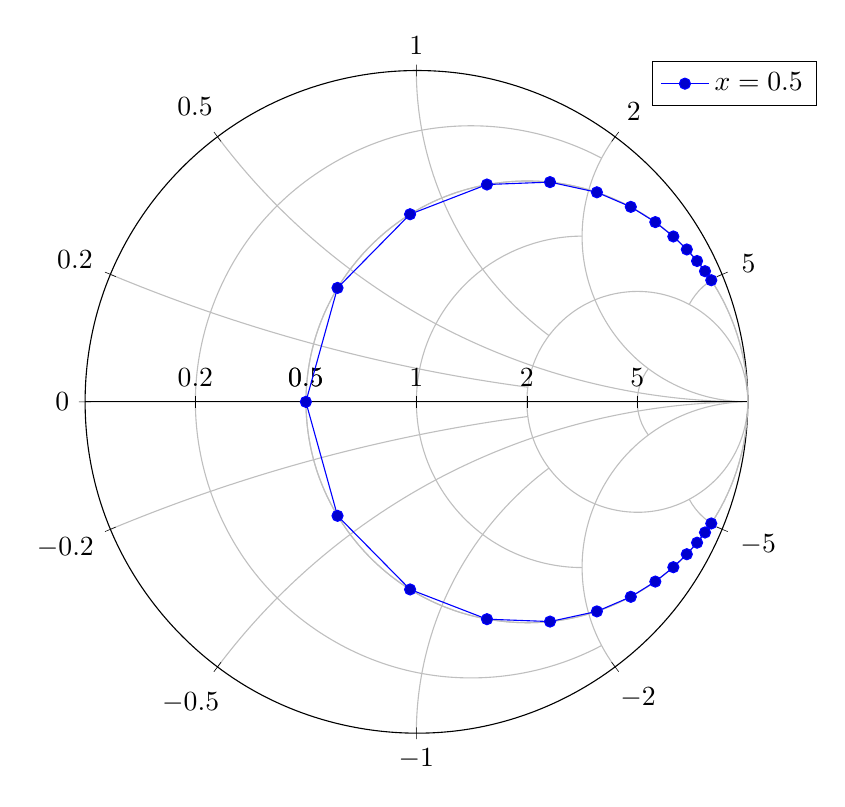
\begin{tikzpicture}
%\tracingmacros=2 \tracingcommands=2
	\begin{smithchartaxis}[
		width=10cm,
		height=10cm,
		xmin=0,xmax=5,
		ymin=-5,ymax=5,
		ygrid each nth passes x={1,2},
		xgrid each nth passes y={2},
	extra x ticks=0.5,
		%xtick={0,30,...,360},
	]
	\addplot+[domain=-5:5] (0.5,\x);
	\addlegendentry{$x=0.5$}
	\end{smithchartaxis}
\end{tikzpicture}
\end{document}
